\section{Thiết kế \& Kết quả (The "How")}

\subsection{Screenshot toàn bộ Dashboard}
\begin{figure}[H]
    \centering
    % \includegraphics[width=\textwidth]{img/dashboard_full.png}
    \caption{Giao diện tổng quan của Dashboard}
\end{figure}

\subsection{Trình bày chi tiết \& Giải thích thiết kế}

\subsubsection{Biểu đồ Nến \& Khối lượng kết hợp Đường Trung bình (MA)}
\begin{figure}[H]
    \centering
    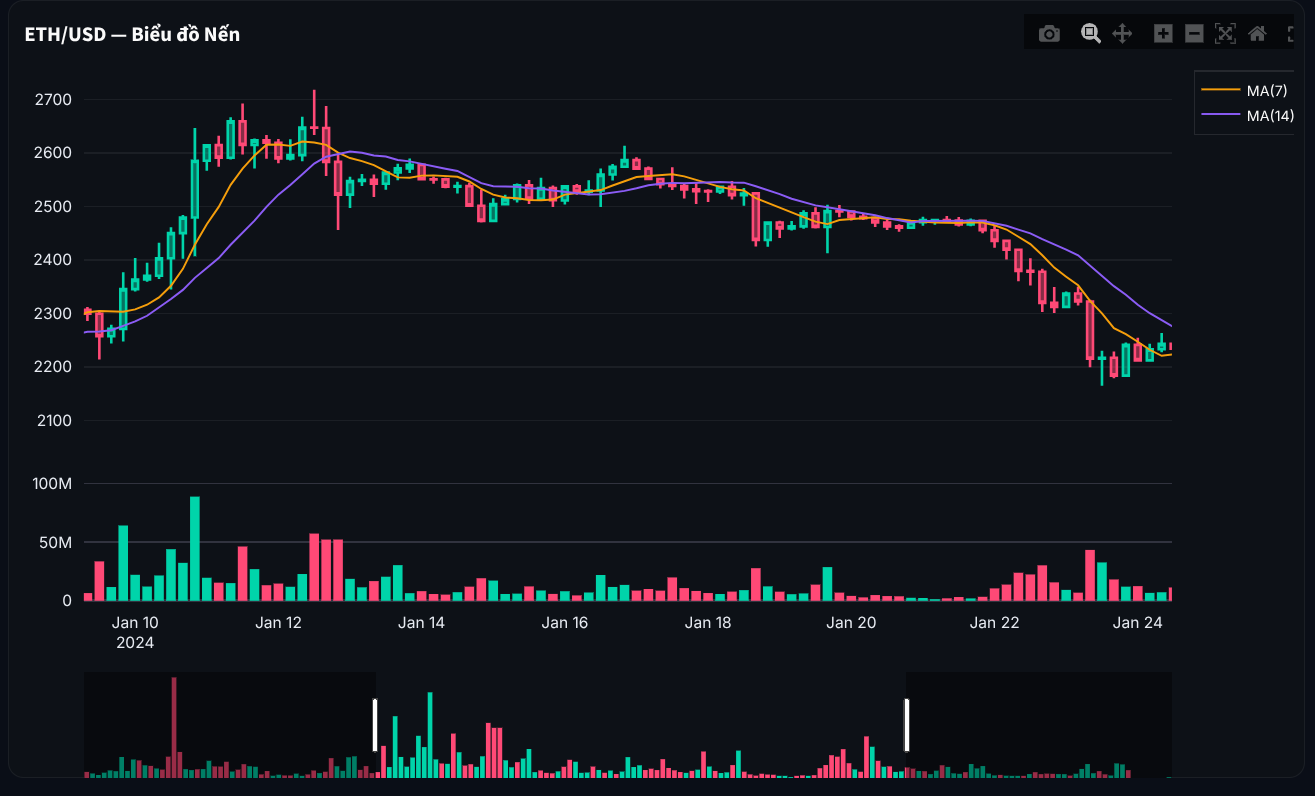
\includegraphics[width=\textwidth]{img/sol_candlestick.png}
    \caption{Biểu đồ nến SOL/USD cùng Khối lượng giao dịch và Đường Trung bình 7 \& 14}
\end{figure}

\textbf{Giải thích thiết kế (Marks \& Channels):}
Dựa trên lý thuyết Trực quan hóa dữ liệu, biểu đồ này sử dụng các Marks (Dấu hiệu) và Channels (Kênh hiển thị) như sau để mã hóa thông tin:

\begin{itemize}
    \item \textbf{Thành phần Nến giá (Candlestick):}
    \begin{itemize}
        \item \textbf{Mark:} Area/Shape (Hình chữ nhật thân nến - Open/Close) và Line (Đường thẳng bóng nến - High/Low).
        \item \textbf{Channel - Vị trí (Position):} Trục X là thời gian, Trục Y là mức giá.
        \item \textbf{Channel - Chiều dài (Size/Length):} Chiều dài thân nến thể hiện độ chênh lệch giữa giá mở cửa và đóng cửa, trong khi thân bóng nến biểu thị biên độ biến động giá trong phiên.
        \item \textbf{Channel - Màu sắc (Color):} Dùng để mã hóa tính chất thay đổi (Kênh Hue). Màu xanh (Identity/Category: Tăng) cho nến đóng cao hơn giá mở, và màu đỏ/hồng cho nến đóng thấp hơn giá mở.
    \end{itemize}
    
    \item \textbf{Thành phần Đường Trung bình động (Moving Average - MA7, MA14):}
    \begin{itemize}
        \item \textbf{Mark:} Line (Đường cong liên tục).
        \item \textbf{Channel - Vị trí (Position):} Trục Y thể hiện mức giá trung bình ứng trên trục X thời gian.
        \item \textbf{Channel - Màu sắc (Color):} Sử dụng màu Cam cho MA(7) và màu Tím cho MA(14). Mục đích cũng là kênh Hue dùng để Phân biệt (Identify) hai chuỗi dữ liệu đường trung bình khác nhau.
    \end{itemize}

    \item \textbf{Thành phần Khối lượng giao dịch (Volume Bar Chart dưới cùng):}
    \begin{itemize}
        \item \textbf{Mark:} Line/Bar (Cột dọc hẹp).
        \item \textbf{Channel - Vị trí (Position):} Đồng bộ trục X thời gian với nến giá phía trên, nhưng trục Y được đặt độc lập thấp bên dưới với thang đo riêng về khối lượng.
        \item \textbf{Channel - Chiều dài (Size/Length):} Chiều cao của cột trên trục Y thể hiện độ lớn định lượng Khối lượng giao dịch.
        \item \textbf{Channel - Màu sắc (Color):} Đồng bộ sắc độ với màu của nến trên cùng khung giờ (xanh hoặc đỏ) để người xem có thể đánh giá nhanh tương quan khối lượng với việc giá tăng/giảm.
    \end{itemize}
\end{itemize}

\textbf{Nhận xét (Insights):}
\begin{itemize}
    \item Xu hướng giá chung từ khoảng 24/Jan/2024 đến 30/Jan/2024 thể hiện đà phục hồi và tăng trưởng của đồng SOL. Đường MA(7) màu cam có xu hướng vượt lên trên đường MA(14) màu tím, xác nhận cấu trúc giao cắt đồng thuận với đà tăng giá ngắn hạn.
    \item Tại các cây nến đỏ sâu trước ngày 24/Jan, cột volume vượt trội cho thấy áp lực bán rát cao. Tuy nhiên, sau vùng giá tạo đáy (ngày 24/Jan), áp lực bán đã suy giảm và lực mua chiếm ưu thế thể hiện qua sự xuất hiện liên tục của các nến xanh thân lớn nhịp nhàng với đà dốc lên của đường MA ngắn hạn.
\end{itemize}
